\section{Introduction}
accumulative model rundown?
Diffusion models of evidence accumulation
Micheyl, Pressnitzer accumulation of adaptation reduces coactivation over time


Is there cumulative history over percept durations for ABA\_ bistability paradigm?

Does it provide a better account of buildup than a model that ignores correlations?

In our previous research, we showed that an alternating renewal process that ignores history dependence and looks only to the steady-state distributions of percept durations does an adequate job of describing transient effects of buildup; this formulation is advantageous because an analytic solution exists to describe the evolution of probability of the split percept from a starting state of grouped, without inferring any global state variable that tracks history across percepts. The dominance durations in most paradigms of bistable perception are well described by gamma density functions, and these have a concise characteristic equation that allows us to solve analytically for the buildup function from steady state dominance durations. However, this simple model may not capture all of the observed behavioral effects; for instance, recent literature has shown weak, but significant, correlations between successive percept durations in the ABA\_ streaming experimental paradigm (Barniv \& Nelken). Furthermore, it does little to constrain potential neuronal mechanisms of alternation. 


Pastukhov \& Braun (2011, 2013) have developed a statistical model for tracking cumulative history across perceptual epochs for perceptual bistability in the visual domain. In this approach, they propose a latent variable, $H_i(t; \tau)$ consisting of a convolution of the perceptual time course of the grouped or split percept ($S_0(t), S_1(t)$) with an exponential filter, $\exp \big [- \frac{(t-t')}{\tau_H} \big ]$, which weights more recent perceptual states more heavily than those further in the past. The variable $H_i(t)$ evolves smoothly over time, increasing in value while the percept it tracks is dominant, and decaying exponentially while the percept is suppressed [FIG]. It takes on values between 0 and 1. Pastukhov \& Braun fitted the parameter $\tau$ so that the correlations of inferred quantities $H_i(t; \tau)$ at the times of switches were maximized with respect to the subsequent percept duration. We took this as a starting point and adapted this measure to be compatible with maximum likelihood methods; thus we are now able to create a full statistical description of how distributions of dominance durations vary with previous history, and can even generate Monte Carlo simulated perceptual timecourses with correlation structure.

[FIG]

This approach allows us to infer the dynamics of history dependence purely by observing the behavioral responses of human listeners in psychoacoustic experimental settings. Merging these techniques with neuronal simulations provides converging evidence for the processes that underlie auditory stream segregation. By combining these statistical methods with human psychophysics and neuromechanistic modeling, we can non-invasively test the neuronal mechanisms that underlie perceptual dynamics; statistics help us to bridge the gap between human behavior and neuronal simulation, and shine a light on the architecture of the auditory system that allows the brain to separate sound sources.

\section{Methods}

Experimental data- 15 subjects, 8 dfs, 3 trials, breakdown of numbers of durations

$S_i(t) \in \{0,1\}$ is a dichotomous variable corresponding to when a listener reports hearing the ambiguous ABA\_ stimulus as grouped ($i=0$) or split ($i=1$). Note that $S_1(t)$ is the same as $Z(t)$ from our previous work examining the buildup of stream segregation (Steele et. al., 2015). Throughout this paper, the time courses of these variables are obtained directly through experiment, or simulated via statistical or neuromechanistic modeling.

Competition models allow us to create data sets with more or less correlation structure 



Cumulative history model: we allow the means of the duration distributions to vary with the previous history computed at the beginning of switch.

\subsection{Analysis}

\subsubsection{Cumulative history function}

The idea of previous history as an exponentially decaying filter on previous states hails from early learning theory (Kamin, Tolman?). The cumulative history function for a particular perceptual state is defined in Pastukhov \& Braun (2011, 2013) as the convolution of the perceptual time course $S(t)$ (which takes on a value of 1 when the percept is dominant, and a value of 0 when the percept is suppressed) with an exponential filter with a time constant, $\tau_h$. It functions as a leaky integrator over previous perceptual states, and is given by

\begin{equation}
\tau_h \frac{dH}{dt} = -H(t) + S(t) \leftrightarrow H(t) = \frac{1}{\tau_H}  \int_0^t S(t') \exp \bigg[- \frac{t-t'}{\tau_H} \bigg] dt'
\end{equation}

We compute $H_i$ analytically in MATLAB from an ordered list of percept durations $T_i, T_j$ with $k$ switches, where $T_i$ is a duration in which the percept tracked by $H_i$ is active and $T_j$ is a duration in which the \textit{other} percept is active. We iteratively solve the integral after each switch time $t_k$: 
\begin{equation*}
\begin{cases}

H_i(t_k) = H_i(t_{k-1}) \exp(- \frac{T_i}{\tau_H}) + (1)  \big(1-\exp(-\frac{T_i}{\tau_H})\big), \\
H_i(t_k) = H_i(t_{k-1}) \exp(- \frac{T_j}{\tau_H}) + (0)  \big(1-\exp(-\frac{T_j}{\tau_H})\big)

\end{cases}
\end{equation*}
We set the values of $H_0(t=0)$ and $H_1(t=0)$ to 0 at the beginning of each trial/ presentation. After an initial transient period, the values of $H_0(t)$ and $H_1(t)$ sum to unity, and are reflections about 0.5. The value of the cumulative history function is dependent on both how long and how recently the percept it tracks was dominant in the past.

\begin{figure}
	\centering
	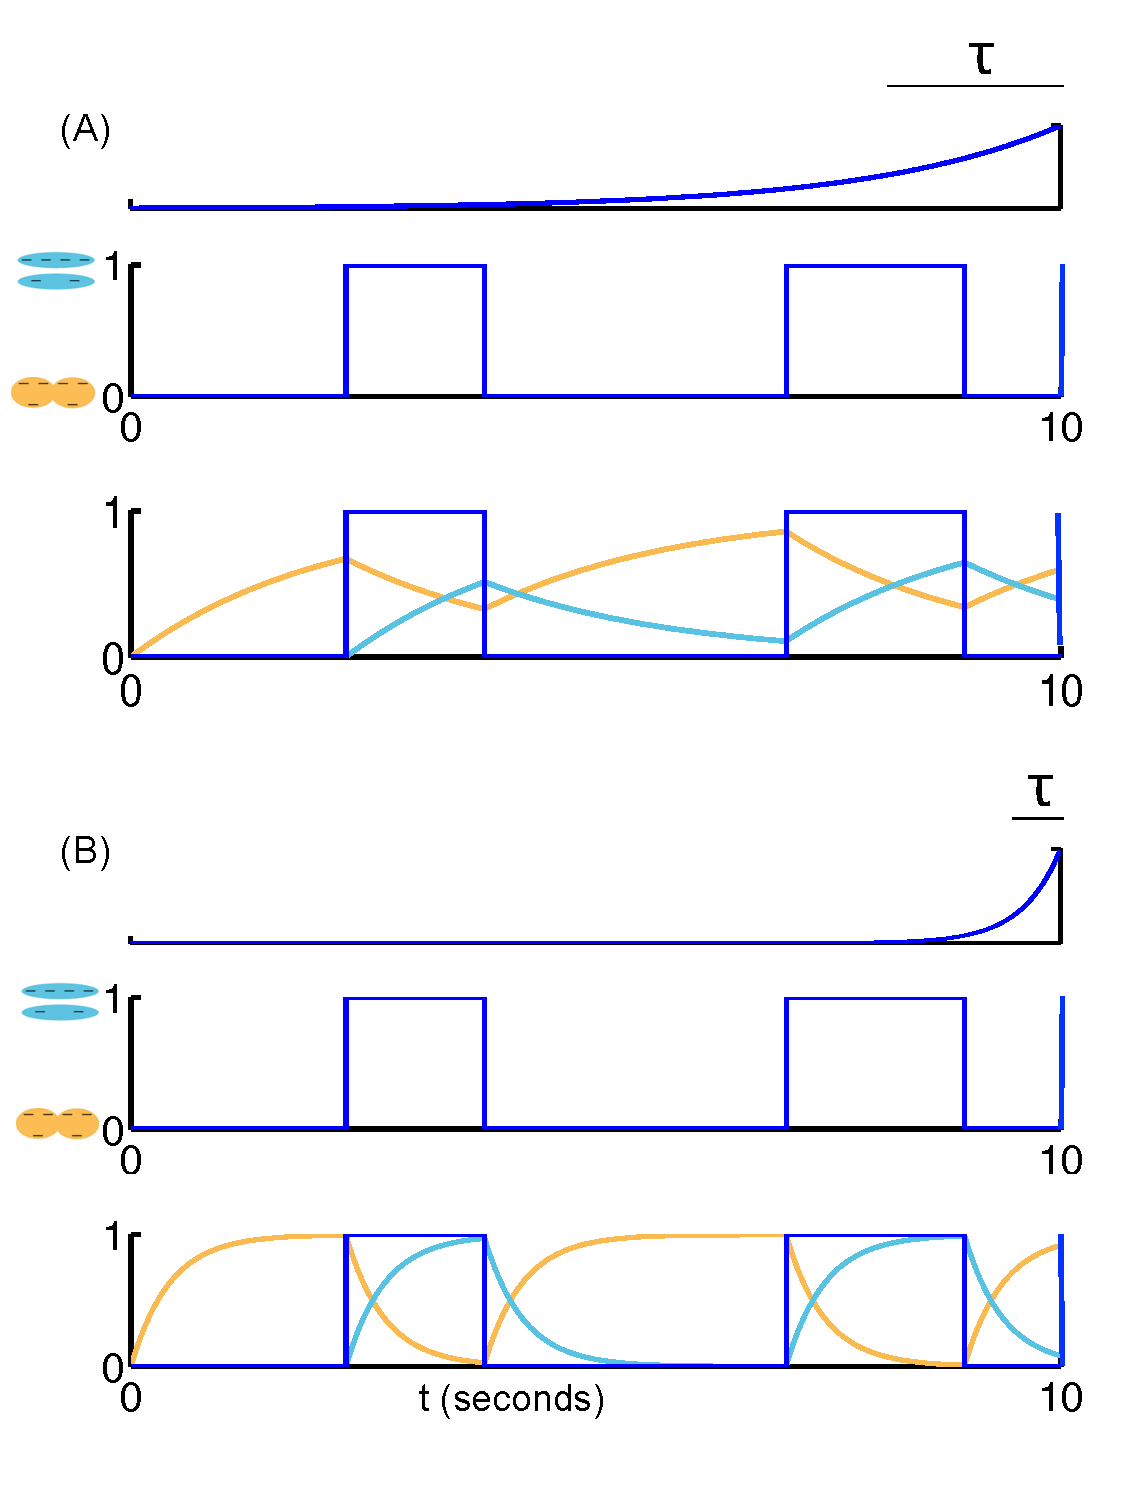
\includegraphics[scale=0.7]{ch3Figs/cumhistPercepts_tau1.pdf}
	\caption{Cumulative history function is a convolution of an exponential filter with a given time scale $\tau$ with the binary perceptual time course. We show the perceptual time course for $S_1(t)$ plotted with $H_0(t)$ (gold) and $H_1(t)$ (blue) for \textbf{(A)} a long time scale, for which the history variable evolves slowly, and \textbf{(B)} a short time scale, for which the history variable evolves and saturates quickly.}
	\label{fig:cumhistPercepts_tau}
\end{figure}

\subsubsection{Full cumulative history model and maximum likelihood estimation}


%Alternative hypothesis- correlations matter; is there history dependence? Does it affect the buildup function? How much data would you need to consider to see a difference?
Our previous model (Steele et. al., 2015) used the steady state distributions of percept durations for grouped and split percepts to describe the dynamics of bistable auditory perception. These were modeled as stationary, independent gamma density functions, parameterized by mean ($\hat{T}$) and shape ($\alpha$) parameters:

\begin{equation}
f(t; \hat{T},\alpha) = \frac{\alpha}{\mu_{T}}\bigg(\frac{\alpha t}{\mu_{T}}\bigg)^{\alpha-1}\bigg(\frac{1}{\Gamma(\alpha)}\bigg)e^{\frac{\alpha t}{\mu_{T}}}
\label{ch3:gamma}
\end{equation}

We use these density functions as a starting point to develop a full generative model. We have developed the cumulative history model of Pastukhov \& Braun (2011, 2013) by allowing the distributions of percept durations to vary as a function of $H(t)$. Specifically, the log of the mean of the gamma density from which a duration is drawn at a switch time depends linearly on the previous history variables at that switch time; this gives a 7 parameter model: fixed shape parameters for the gamma densities for each percept $\alpha_0, \alpha_1$, the intercept $\beta_0, \beta_1$, (mean duration at H=0), the slope $m_0, m_1$ (how log mean duration varies with H), and $\tau_h$, the timescale of the cumulative history accumulation. The gamma density describing the \textit{next} duration $T_i $ is a function of the value of the value of $H_i (t_k)$ at the time of switching into that interval; specifically, we keep the same shape parameter for all intervals and allow the mean to vary according to

\begin{equation}
\ln \mu_{T_i} = \beta_i + m_i H_i(t_k)
\end{equation}

Note that we use $\mu_{T_i}$ to describe the mean of the gamma density at a particular $H_i$ value, and $\hat{T}$ to describe the sample mean of durations of the same type over the course of the whole trial. 

We use maximum likelihood methods to recover the parameters of Monte Carlo simulated data. We compute the likelihood of a a data set for a given set of parameters iteratively; after each switch time, we computed the value of $H(t)$ for each percept. The value of $H(t)$ set the distribution for the next percept $p(T_i|H(t))$. Each set of parameters defines a family of density functions, from which the likelihood of a given trial time course can be computed exactly. We found parameters for each subject/condition that maximized the sum of the log of the likelihoods of the durations reported by that subject in that condition. 


; we also use neuronal competition models previously developed to describe perceptual bistability.% to see how much data we need to find a good fit for both adaptation-driven switching (for which correlations are high and the cumulative history should have a significant effect on the subsequent durations) as well as noise-driven switching (for which correlations are low and cumulative history should not have a significant effect). 
We then do model comparison between the 7 parameter cumulative history model and the 4 parameter ARP model using Wilks' theorem likelihood ratio test.

\subsubsection{Correlations}

Because every data set contains two percept types, we wanted to have a consistent, simple way to determine whether any given trial time course contained significant correlations. We used the Fisher $z$-transformation (arctanh($r$) $ = \frac{1}{2} \ln \frac{1 + x} {1 - x}$) to convert Pearson's sample correlation coefficient $r$, and divided by the standard error $1/\sqrt{N-3}$ to obtain $Z$-scores; under the null hypothesis of zero correlation, any two random variables will have a standard normal distribution of arctanh($r$)$\sqrt{N-3}$.
We confirmed with Monte Carlo simulations of independent gamma distributed samples that for the null hypothesis of no correlation, the pair of $Z$-scores would be distributed according to an independent bivariate normal distribution. We created a measure $\rho$ according to the distance of this pair of $Z$-scores from the origin: 

\begin{equation}
\hat{\rho} = \sqrt{z_1^2 + z_2^2}
\end{equation}

This allowed us to identify data sets with significant correlations. We confirmed these with permutation tests (Supplemental) and found similar p-values. Because the number of durations in each trial was small and because the data are not normally distributed, we used assumption-free resampling methods to determine whether the correlations were significant. For all subjects except for one, there were moderate, significant, positive correlations between successive percept durations of alternate types. We constructed a distribution of correlation coefficients for the null hypothesis rho = 0 by scrambling the intervals of one type for each subject. Permutation tests of this type are very robust at controlling Type I errors in non-normal data (Bishara and Hittner, 2012). 

%How can we combine data across subjects to get buildup functions and distributions?

\section{Results}

%for subjects and conditions with a good number of durations, we see good agreement between buildup functions and ARP predictions from gamma densities.

%We know from our last paper (ie Figure 5) that there are deviations from ARP for the models that produce significant correlations—-- we want to quantify these deviations and determine how large a role they play for the psychophysical data

%We have previously applied the cumulative history model using a method to fit it to data by maximizing the correlation between the H function (with a certain tau) and the subsequent duration; however, the results using this method have been inconsistent [SUPPLEMENTAL] and we have switched to a maximum likelihood approach to estimating the parameters of the cumulative history function.

We know that the correlation structure in ambiguous perception varies significantly between different stimulus conditions and also between different listeners. Since every data set has two types of transitions (Integration-Segregation and Segregation-Integration) we wanted a way to combine the correlation coefficients to be able to say whether a given set of samples displays correlations beyond those expected to be observed by chance from a data set. 

\subsection{Data have serial correlations- these are usually significant for conditions around equidominance}

We wanted to see if we could detect correlations between subsequent percept durations in our data. For each subject, we computed the correlation coefficient for I->S transitions and S->I transitions separately. We also computed the combined correlation coefficient Rho 


\begin{figure}
	\centering
	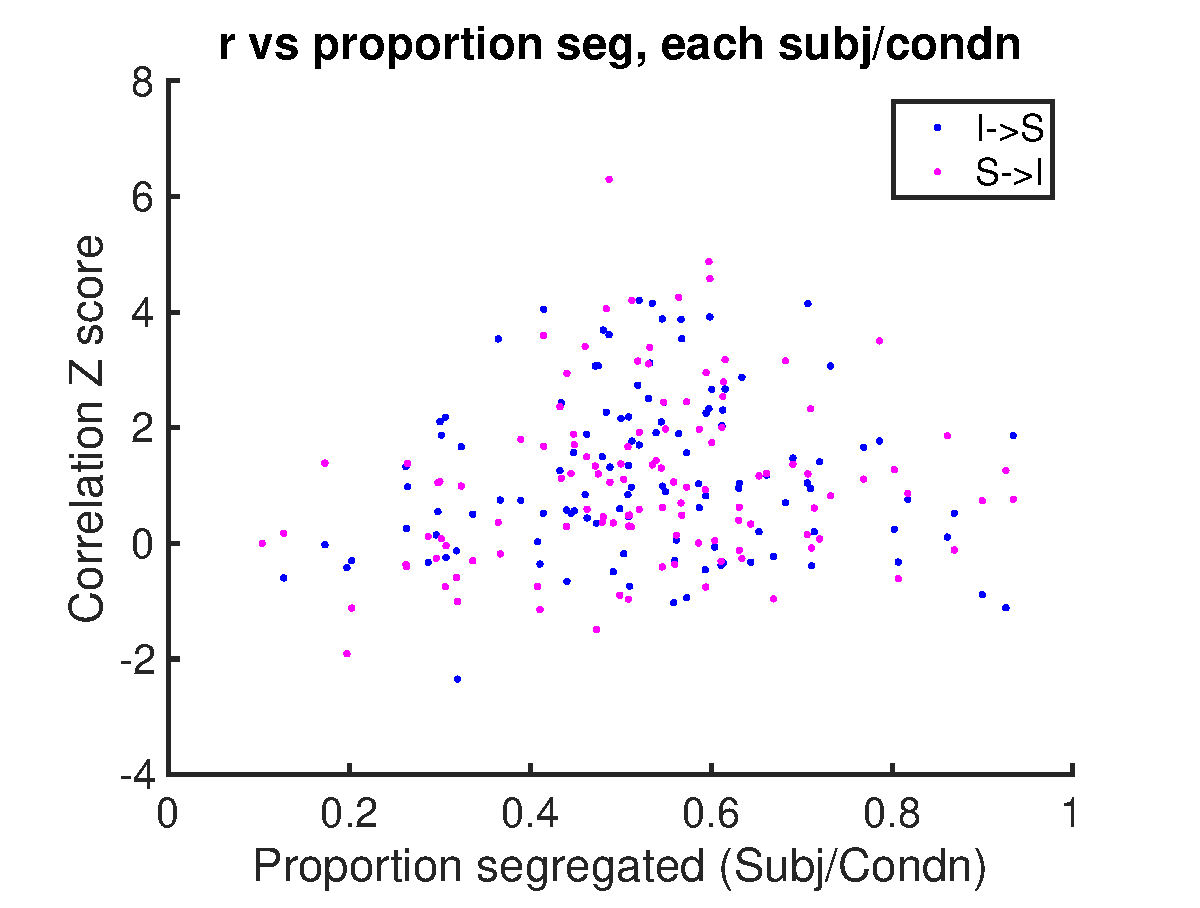
\includegraphics[scale=0.7]{ch3Figs/SC_rz_vs_propSplit.eps}
	\caption{help}
	\label{fig:SC_rz_vs_propSplit}
\end{figure}


\subsection{We are able to recover the parameters from the generative model using MLE}

Many data sets do not show significant cumulative history; those which do show a strong effect of cumulative history are predominantly from experimental conditions that produce equidominance, in which the auditory stimulus is near perfectly ambiguous and integration and segregation have equal mean durations throughout the trial. Because the time scale of cumulative history is typically shorter than a single perceptual epoch, it is difficult to observe for conditions in which one percept is much longer than another; over a long epoch, the accrual of noise drowns out the effects of previous history. Data sets for which cumulative history gives significant correlations with successive perceptual epochs also often demonstrated marginally significant serial correlations.

We did not attempt to fit the history model to data sets for which fewer than 20 durations were observed. Six of the 120 subject/condition data sets were excluded for this reason.

We found significant correlations between cumulative history and next percept duration for 40 out of 120 data sets. 23 out of 114 data sets recovered $\tau_{H}$ less than 0.2 seconds; 4 of these gave significant correlations between $H$ and $T_{next}$. Because these would not meaningfully elucidate the role of cumulative history across percepts, they were excluded from further analysis.

Tau that maximized R was also computed; typically, this was close to the value found by MLE. 

\subsection{Durations vary systematically with the fitted history values in experimental data}

When we examined all the data sets with significant correlations between the cumulative history $H(t)$ at switch times $(t_k)$ and next percept durations $T$, we saw a striking relationship \ref{fig:T_vs_H}. For each data set, we binned over the values of $H(t)$ computed at switch times and examined whether the percept durations following were longer or shorter than their mean values. The $H$ functions for each percept type, integration or segregation, both start at 0 and then proceed to a steady state where their values sum to one. Thus, there is a “transient” phase, during which the sum of $H_0(t)$ and $H_1(t)$ is less than one, and a steady state where each H function is a mirror image of the other about 0.5, such that they sum to unity. Depending on the $\tau$ (which controls how fast the history function saturates) this could take 10 s to over a  minute. For the values of $H$ we observed at steady state, we found a very striking dependency. The average durations $\mu_{T_i}$ of the percepts following the value of $H_i$ at a switch time were significantly different in a predictable, systematic way, dependent on the particular value of $H(t)$--- there was a negative relationship between the cumulative history of a given percept and the durations of that percepts in the subsequent interval. Durations following a mid-trial switch in which the value of $H(t_k)$ was near 0 (such as when the intervening alternate percept was very long) were nearly twice as long as their trial mean value, whereas durations following an $H(t_k)$ value near 1 were just over half their “typical” value, $\mu_{T}$.

\begin{figure}
	\centering
	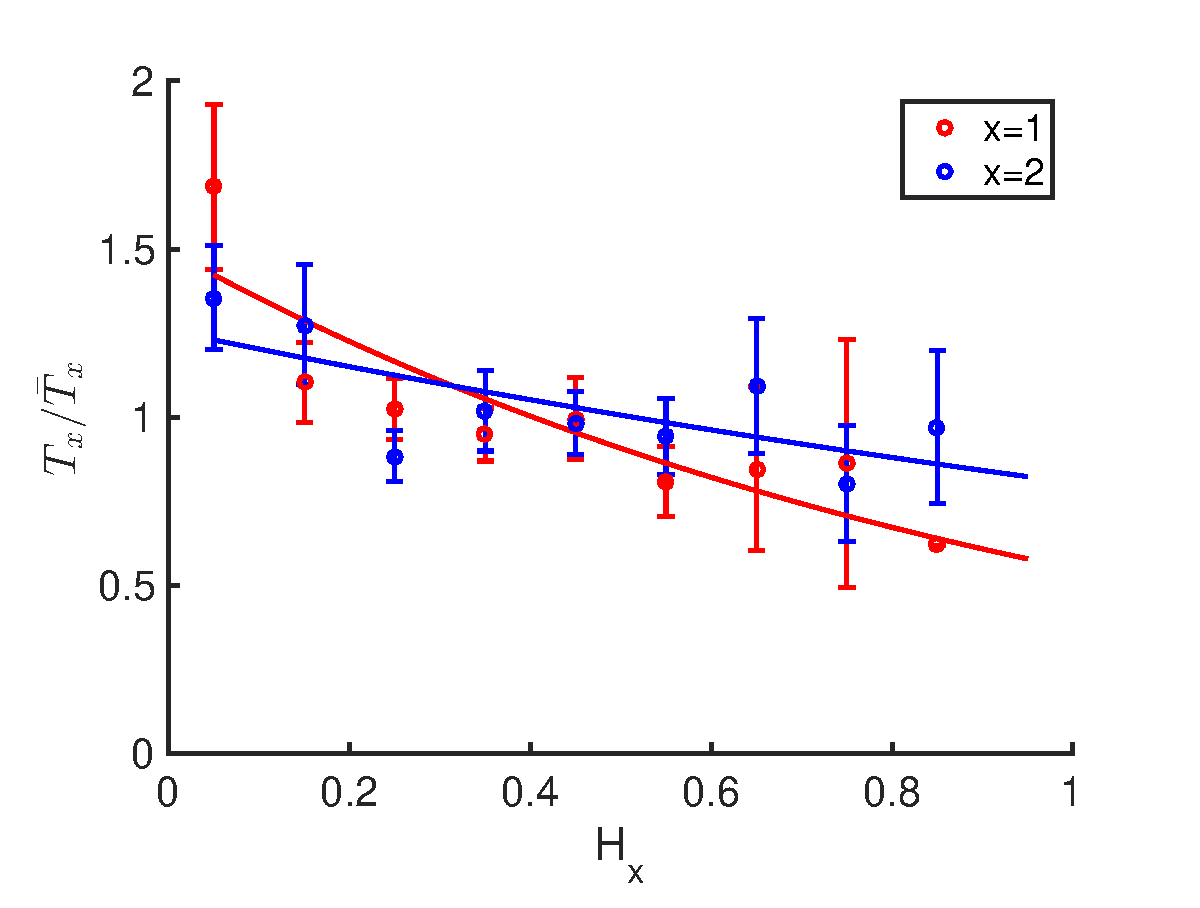
\includegraphics[scale=0.7]{ch3Figs/tbyh.eps}
	\caption{christ}
	\label{fig:T_vs_H}
\end{figure}

This may partially account for the phenomenon of “inertia” in bistable perception, in which the first percept of a trial is typically longer than the other percepts of the same type. While previously reported levels of inertia in other bistable streaming stimuli were at the level of an order of magnitude longer initial percepts, we observed inertia at a level of roughly twice as long initial percept. If one assumes that the history function would be at a value near zero for the beginning of the trial, it makes sense to look the durations of percepts at steady state that occur when the value of the history function at a switch is close to zero to see if they are similarly long. We observed a ratio of ~1.7 over the mean for percepts in the middle of the trial with these history values at the switch time.

This non-stationarity can only be observed by invoking an inferred quantity, $H(t; \tau)$ that is fitted through maximum likelihood estimation for each subject and condition. The values of $\tau$ are not consistent across subjects; [WHAT WOULD HELP FIND CONSISTENCY? DO SUBJS HAVE RHYME OR REASON TO WHEN THEY HAVE SIG CORRS WITH H AND T?]

DO SUBJECTS SHOW SAME TAU VALUES OVER DIFFERENT CONDITIONS?

\subsection{Cumulative history model that only sees behavioral responses uncovers hidden parameters in neuronal simulations}

We used as a test bed the neuronal competition models outlined in Shpiro et. al., which allow us to modulate the role of adaptation and to control the correlation structure. We know that higher gain on adaptation produces percept durations that are more strongly correlated. We expected that the ability to fit the cumulative history model (find a $\tau$ that maximizes $\hat{\rho}$) would differ between dynamical regimes where adaptation was the primary mechanism of alternation versus those with noise-driven switching; however, this was not the case \ref{fig:rho_vs_tau_ax}. While the recovered maximum correlations were weaker for attractor models, in which switches between perceptual states were driven by noise, even weak adaptation allowed us to consistently fit a $\tau_H$. When adaptation is abolished completely, no significant correlations are found and the tau that maximizes $\hat{\rho}$ comes out different every time.

\begin{figure}
	\centering
	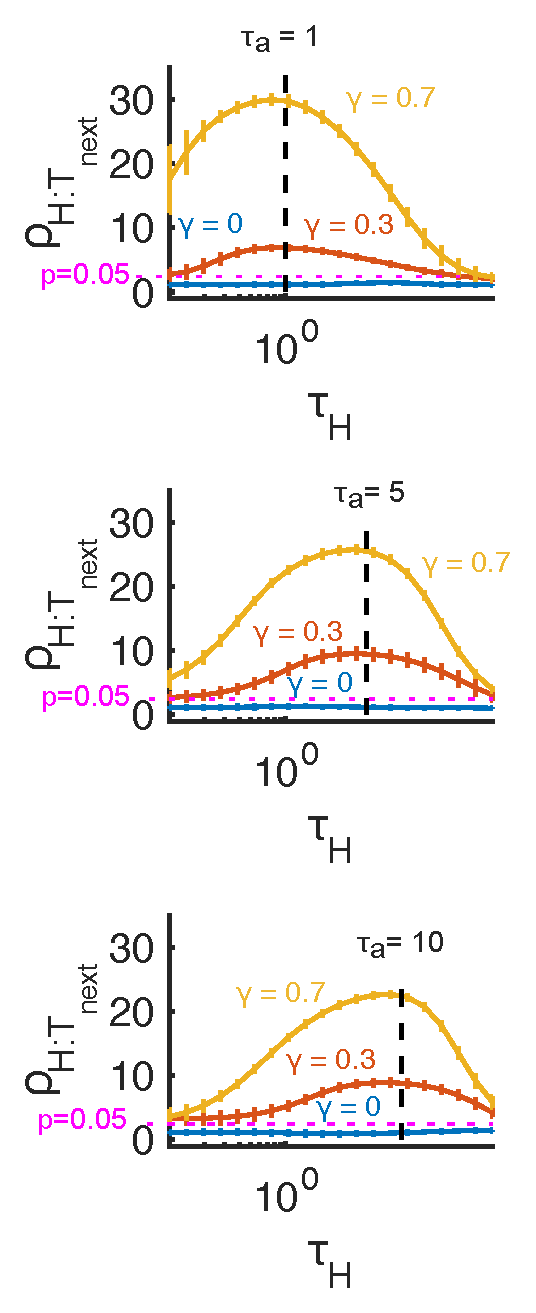
\includegraphics[scale=0.65]{ch3Figs/rho_vs_tau_sim_edit.pdf}
	\caption{The value of $\tau_H$ that maximizes the correlation between cumulative history and dominance durations in neuronal competition model simulations varies with the underlying neuronal time scale. We computed the combined correlation $\hat{\rho}$ for simulations of duration 4800 s with leaky oscillator dynamics using strong adaptation, ($\gamma = 0.7$, yellow curves), with attractor dynamics using weak adaptation ($\gamma = 0.3$, red curves), and with no adaptation ($\gamma = 0$, blue curves). Each plot shows a different timescale of adaptation-- $\tau_a$ = 1 s (top), $\tau_a$ = 5 s (middle) and $\tau_a$ = 10 s (bottom). We show the correlation at each value of $\tau_H$. While we found no effect of cumulative history on subsequent dominance durations for simulations that had no adaptation, we found significant correlations for both oscillator and attractor dynamics, and these peaked at or near the value of the underlying adaptation time constant. We performed each set of simulation parameters and correlation computations 10 times.}
	\label{fig:rho_vs_tau_ax}
\end{figure}


We compared virtual listeners with neurophysiological simulations operating under three dynamical regimes-- one with zero adaptation (a purely Poisson process, a true alternating renewal process), one with weak adaptation (an attractor with mild fluctuations in energy wells, but with switches between states driven by noise) and a leaky oscillator (with an underlying periodic rhythm in switches between perceptual state). For both models with adaptation, even when switches were not driven by noise, we found that the value of $\tau_H$ that maximized the correlation between the cumulative history value $H$ at a switch time $t_k$ and the subsequent durations would vary directly with the underlying adaptation time constant used in the simulation. We used simulations at equidominance, which corresponds to those behavioral conditions that maximized serial correlations between percept durations. The value of $\tau_H$ that maximized predictive value of the next percept duration was very close to the actual value of the neurophysiological time constant used in the simulations.

One might surmise that this allows us to determine on a subject by subject basis what the underlying time constant of neuronal adaptation for auditory stream segregation is; however, there are some practical difficulties with ascertaining this. First, the simulations we used were the equivalent of 20 four minute trials in one condition. The most data we collected for any of our subjects was 5 blocks. Furthermore, neuronal adaptation might operate on different time scales for different stimulus conditions; while we observed subjects who were "fast" and "slow" switchers, they displayed a wide range of fitted time constants. However, we believe that by learning the time constant of cumulative history, we can develop a behavioral proxy for the adaptation state of the neural circuits that underlie auditory scene analysis. In our simulations, when we measured the state of the adaptation variable $a$ at a switch time, it was highly correlated to the value of the cumulative history variable $H$. 

\subsubsection{Simulated distributions are consistent with those predicted by the cumulative history model}
By fitting the cumulative history model, we can compute both the value of H at every switch time, as well as the expected distribution of durations for that $H$ value (because the distributions vary lawfully as a function of $H(t_k)$. When we bin over computed values of $H(t_K)$s and look at histograms of the simulated durations in the different bins, we find very good correspondence between the actual and the expected duration distributions. The degree to which the means of these duration distributions shifted at different observed values of $H$, i. e., the sensitivity to cumulative history, did not vary significantly between different dynamical regimes.

While the reliability of the cumulative history model does not distinguish between dynamical regimes, the $\tau$ values recovered by maximum likelihood estimation of the parameters of the cumulative history model are typically very close to the timescale of adaptation specified in the neuronal competition model. When the adaptation time constant is 2 seconds, for instance, the recovered tau for the cumulative history model is consistently near 2 seconds for all dynamical regimes tested so far. When the adaptation time constant is 10 seconds, the recovered tau for the cumulative history model is consistently near 10 seconds.

FURTHERMORE THESE ARE BETTER ABLE TO DESCRIBE THE TIMECOURSE OF HUMAN EXPERIMENTS (LL TEST) AND WE ARE ABLE TO RECREATE SIMULATED TIMECOURSES WITH THE STATISTICAL MODEL THAT HAVE SIMILAR DISTRIBUTIONS TO THE ORIGINAL DATA (HISTS VS H)

\subsection{Buildup functions}

Because we have full generative models that either do or do not take history dependence into account, we can produce simulated listeners that either do or do not display history dependence in Monte Carlo. From these simulated listeners’ simulated responses, we can construct buildup functions, and also estimate the 95\% confidence bounds on 1000s of simulated buildup functions from each process. We can then compare the buildup functions from the cumulative history model to those from the ARP, as well as the true buildup functions, to determine whether a model that considers cumulative history makes better predictions than that which does not. This is evaluated through accuracy ($R^2$ between the average and the true buildup function) or precision (smaller confidence intervals).

\subsection{Discussion}

Relationship between H and the adaptation variable in competition model simulations? We believe that our model bridges a gap between explaining physiological processes (which are difficult to directly characterize for ambiguous perceptual phenomena, as subjects must report their perception continuously while their brains are recorded) and the observed statistics of listeners' behavior. By estimating the parameters of the statistical model, we can both describe and predict future behavior, as well as make inferences about the underlying neuronal processes. Specifically, we believe that our statistically derived $H$ variable is a proxy for the level of adaptation in the underlying neuronal populations. The relationship between the $H$ value at a switch time and the duration of the subsequent perceptual epoch is to characterize the transition of a suppressed state $j$ to a dominant one. The formerly suppressed state has been recovering from adaptation before the switch; the longer it has been suppressed, the lower the value of $H_j$ (and, as we understand neural processes, adaptation). Therefore, we would expect the next duration to be longer if the $H$ value is low, and shorter if the $H$ value is high-- hence the negative slope observed for $ln(T_j)$ vs. $H_j$.

% How much data do we need for the 7 parameter model to provide a better account (by likelihood ratio) than the 4 parameter model, for different underlying processes in the competition model? Criterion: > 2 log lik(cumhist)/ lik(ARP) ~ Chi square, 3 degrees of freedom. How does this translate to the human data?

Perturbation study- once we fit the tau for a given listener/condition, we can make an online computation of what the value of their history function should be, and exploit the added information we would have at every switch for predicting the length of the next interval. We can also treat H as a proxy for the underlying adaptation variable. 
